

\begin{figure*}[t]
    \centering
    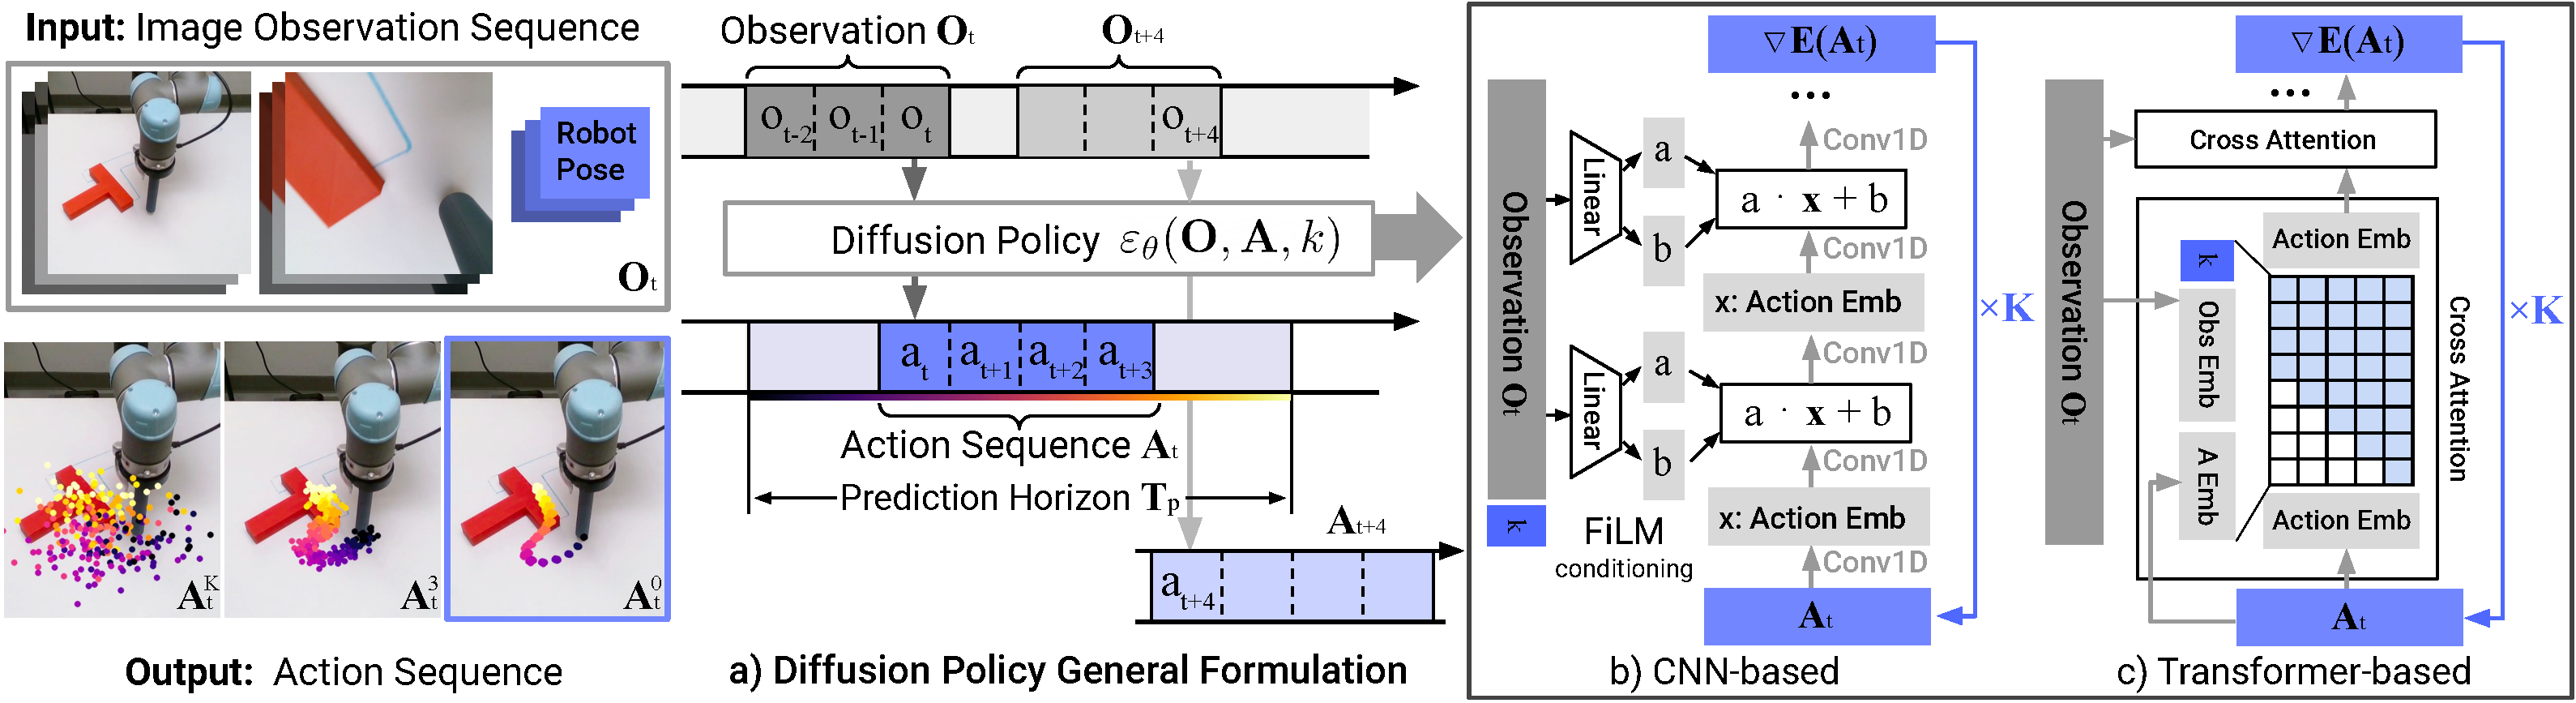
\includegraphics[width=\linewidth]{figure/policy_input_output.pdf}
    \caption{\textbf{Diffusion Policy Overview} \label{fig:policy_io} a) General formulation. At time step $t$, the policy takes the latest $T_o$ steps of observation data $O_t$ as input and outputs $T_a$ steps of actions $A_t$.  b) In the CNN-based Diffusion Policy, FiLM (Feature-wise Linear Modulation) \cite{perez2018film} conditioning of the observation feature $O_t$ is applied to every convolution layer, channel-wise. Starting from $\mathbf{A}^K_t$ drawn from Gaussian noise, the output of noise-prediction network $\epsilon_\theta$ is subtracted, repeating $K$ times to get $\mathbf{A}^0_t$, the denoised action sequence. c) In the Transformer-based \cite{vaswani2017attention} Diffusion Policy, the embedding of observation $\mathbf{O}_t$ is passed into a multi-head cross-attention layer of each transformer decoder block. Each action embedding is constrained to only attend to itself and previous action embeddings (causal attention) using the attention mask illustrated.  }
\end{figure*}

\section{Diffusion Policy Formulation}
\label{sec:method}

We formulate visuomotor robot policies as Denoising Diffusion Probabilistic Models (DDPMs) \cite{ho2020denoising}. Crucially, Diffusion policies are able to express complex multimodal action distributions and possess stable training behavior -- requiring little task-specific hyperparameter tuning.
The following sections describe DDPMs in more detail and explain how they may be adapted to represent visuomotor policies.

\subsection{Denoising Diffusion Probabilistic Models}
\label{sec:ddpm}
DDPMs are a class of generative model where the output generation is modeled as a denoising process, often called Stochastic Langevin Dynamics \cite{welling2011bayesian}.

Starting from $\mathbf{x}^K$ sampled from Gaussian noise, the DDPM performs $K$ iterations of denoising to produce a series of intermediate actions with decreasing levels of noise,
$\mathbf{x}^k, \mathbf{x}^{k-1} ...\mathbf{x}^{0} $, until a desired noise-free output $\mathbf{x}^0$ is formed.
The process follows the equation
\vspace{-1mm}
\begin{equation}
    \textbf{x}^{k-1}=\alpha(\textbf{x}^{k}-\gamma\epsilon_\theta(\mathbf{x}^k,k) + \mathcal{N} \bigl(0, \sigma^2 I \bigl)),
    \label{eq:unconditional_langevin}
\vspace{-1mm}
\end{equation}
where $\epsilon_\theta$ is the noise prediction network with parameters $\theta$ that will be optimized through learning and $\mathcal{N} \bigl(0, \sigma^2 I \bigl)$ is Gaussian noise added at each iteration.


The above equation \ref{eq:unconditional_langevin} may also be interpreted as a single noisy gradient descent step:
\vspace{-2mm}
\begin{equation}
    \mathbf{x}'=\mathbf{x}-\gamma\nabla E(\mathbf{x}),
    \label{eq:gradient_descent}
\vspace{-1mm}
\end{equation}
where the noise prediction network $\epsilon_\theta(\mathbf{x},k)$ effectively predicts the gradient field $\nabla E(\mathbf{x})$, and  $\gamma$ is the learning rate.

The choice of $\alpha,\gamma,\sigma$ as functions of iteration step $k$, also called noise schedule, can be interpreted as learning rate scheduling in gradient decent process.
An $\alpha$ slightly smaller than $1$ has been shown to improve stability \cite{ho2020denoising}.
Details about noise schedule will be discussed in Sec \ref{sec:method-noise-schedule}.


\subsection{DDPM Training}
\label{sec:ddpm_inference}


The training process starts by randomly drawing unmodified examples, $\mathbf{x}^0$, from the dataset. For each sample, we randomly select a denoising iteration $k$ and then sample a random noise $\mathbf{\epsilon}^k$ with appropriate variance for iteration $k$. The noise prediction network is asked to predict the noise from the data sample with noise added.

\vspace{-2mm}
\begin{equation}
    \mathcal{L} = MSE(\mathbf{\epsilon}^k, \epsilon_\theta(\mathbf{x}^0+\mathbf{\epsilon}^k,k))
    \label{eq:unconditional_loss}
\end{equation}

As shown in \cite{ho2020denoising}, minimizing the loss function in Eq \ref{eq:unconditional_loss} also minimizes the variational lower bound of the KL-divergence between the data distribution $p(\mathbf{x}^0)$ and the distribution of samples drawn from the DDPM $q(\mathbf{x}^0)$ using Eq \ref{eq:unconditional_langevin}.







\subsection{Diffusion for Visuomotor Policy Learning}

While DDPMs are typically used for image generation ($\mathbf{x}$ is an image), we use a DDPM to learn robot visuomotor policies. This requires two major modifications in the formulation:
1. changing the output $\mathbf{x}$  to represent robot actions.
2. making the denoising processes \textit{conditioned} on input observation $\mathbf{O}_t$.
The following paragraphs discuss each of the modifications, and Fig. \ref{fig:policy_io} shows an overview.

\textbf{Closed-loop action-sequence prediction:}
An effective action formulation should encourage temporal consistency and smoothness in long-horizon planning while allowing prompt reactions to unexpected observations.
To accomplish this goal, we commit to the action-sequence prediction produced by a diffusion model for a fixed duration before replanning.
Concretely, at time step $t$ the policy takes the latest $T_o$ steps of observation data $\mathbf{O}_t$ as input and predicts $T_p$ steps of actions, of which $T_a$ steps of actions are executed on the robot without re-planning. Here, we define $T_o$ as the observation horizon, $T_p$ as the action prediction horizon and $T_a$ as the action execution horizon.
This encourages temporal action consistency while remaining responsive. More details about the effects of $T_a$ are discussed in Sec \ref{sec:action_sequence}.
Our formulation also allows receding horizon control \cite{mayne1988receding} to futher improve action smoothness by warm-starting the next inference setup with previous action sequence prediction.




\textbf{Visual observation conditioning:}
We use a DDPM to approximate the conditional distribution $p(\mathbf{A}_t | \mathbf{O}_t)$ instead of the joint distribution $p(\mathbf{A}_t,\mathbf{O}_t)$ used in \citet{janner2022diffuser} for planning. This formulation allows the model to predict actions conditioned on observations without the cost of inferring future states, speeding up the diffusion process and improving the accuracy of generated actions.
To capture the conditional distribution $p(\mathbf{A}_t |\mathbf{O}_t)$, we modify Eq \ref{eq:unconditional_langevin} to:
\begin{equation}
    \label{eq:diffusion_policy_langevin}
    \mathbf{A}^{k-1}_t = \alpha(\mathbf{A}^k_t - \gamma\epsilon_\theta(\mathbf{O}_t,\mathbf{A}^k_t,k) + \mathcal{N} \bigl(0, \sigma^2 I \bigl))
\end{equation}
The training loss is modified from Eq \ref{eq:unconditional_loss} to:
\begin{equation}
    \label{eq:diffusion_policy_loss}
    \mathcal{L}=MSE(\mathbf{\epsilon}^k,\epsilon_\theta(\mathbf{O}_t, \mathbf{A}^0_t + \mathbf{\epsilon}^k, k))
\end{equation}

The exclusion of observation features $\mathbf{O}_t$ from the output of the denoising process significantly improves inference speed and better accommodates real-time control. It also helps to make \textbf{end-to-end} training of the vision encoder feasible.
Details about the visual encoder are described in Sec. \ref{sec:method-visual}.














\section{Key Design Decisions}
 In this section, we describe key design decisions for Diffusion Policy as well as its concrete implementation of $\epsilon_\theta$ with neural network architectures.

\subsection{Network Architecture Options}
\label{sec:method-network}
The first design decision is the choice of neural network architectures for $\epsilon_\theta$.
In this work, we examine two common network architecture types, convolutional neural networks (CNNs) \cite{ronneberger2015u} and Transformers \cite{vaswani2017attention}, and compare their performance and training characteristics. Note that the choice of noise prediction network $\epsilon_\theta$ is independent of visual encoders, which will be described in Sec. \ref{sec:method-visual}.

\textbf{CNN-based Diffusion Policy}
We adopt the 1D temporal CNN from \citet{pmlr-v162-janner22a} with a few modifications:
First, we only model the conditional distribution $p(\mathbf{A}_t|\mathbf{O}_t)$ by conditioning the action generation process on observation features $\mathbf{O}_t$ with Feature-wise Linear Modulation (FiLM) \cite{perez2018film} as well as denoising iteration $k$, shown in Fig \ref{fig:policy_io} (b).
Second, we only predict the action trajectory instead of the concatenated observation action trajectory.
Third, we removed inpainting-based goal state conditioning due to incompatibility with our framework utilizing a receding prediction horizon. However, goal conditioning is still possible with the same FiLM conditioning method used for observations.

In practice, we found the CNN-based backbone to work well on most tasks out of the box without the need for much hyperparameter tuning. However, it performs poorly when the desired action sequence changes quickly and sharply through time (such as velocity command action space), likely due to the inductive bias of temporal convolutions to prefer low-frequency signals \cite{tancik2020fourier}.

\textbf{Time-series diffusion transformer}
To reduce the over-smoothing effect in CNN models \cite{tancik2020fourier}, we introduce a novel transformer-based DDPM which adopts the transformer architecture from minGPT \cite{bet} for action prediction.
Actions with noise $A_t^k$ are passed in as input tokens for the transformer decoder blocks, with the sinusoidal embedding for diffusion iteration $k$ prepended as the first token.
The observation $\mathbf{O}_t$ is transformed into observation embedding sequence by a shared MLP, which is then passed into the transformer decoder stack as input features.
The ``gradient" $\epsilon_\theta(\mathbf{O_t},\mathbf{A_t}^k,k)$ is predicted by each corresponding output token of the decoder stack.

In our state-based experiments, most of the best-performing policies are achieved with the transformer backbone, especially when the task complexity and rate of action change are high. However, we found the transformer to be more sensitive to hyperparameters. The difficulty of transformer training \cite{liu2020understanding} is not unique to Diffusion Policy and could potentially be resolved in the future with improved transformer training techniques or increased data scale.

\textbf{Recommendations.}
 In general, we recommend starting with the CNN-based diffusion policy implementation as the first attempt at a new task. If performance is low due to task complexity or high-rate action changes, then the Time-series Diffusion Transformer formulation can be used to potentially improve performance at the cost of additional tuning.

\subsection{Visual Encoder}
\label{sec:method-visual}
The visual encoder  maps the raw image sequence into a latent embedding $O_t$ and is trained end-to-end with the diffusion policy.
Different camera views use separate encoders, and images in each timestep are encoded independently and then concatenated to form $O_t$.
We used a standard ResNet-18 (without pretraining) as the encoder with the following modifications:
1) Replace the global average pooling with a spatial softmax pooling to maintain spatial information \cite{robomimic}.
2) Replace BatchNorm with GroupNorm \cite{groupnorm} for stable training. This is important when the normalization layer is used in conjunction with Exponential Moving Average \cite{he2020moco} (commonly used in DDPMs).

\subsection{Noise Schedule}
\label{sec:method-noise-schedule}
The noise schedule, defined by $\sigma$, $\alpha$, $\gamma$ and the additive Gaussian Noise $\epsilon^k$ as functions of $k$, has been actively studied \cite{ho2020denoising, nichol2021improved}.  The underlying noise schedule controls the extent to which diffusion policy captures high and low-frequency characteristics of action signals. In our control tasks, we empirically found that the Square Cosine Schedule proposed in iDDPM \cite{nichol2021improved} works best for our tasks.

\subsection{Accelerating Inference for Real-time Control}
We use the diffusion process as the policy for robots; hence, it is critical to have a fast inference speed for closed-loop real-time control. The Denoising Diffusion Implicit Models (DDIM) approach \cite{song2021ddim}  decouples the number of denoising iterations in training and inference, thereby allowing the algorithm to use fewer iterations for inference to speed up the process. In our real-world experiments, using DDIM with 100 training iterations and 10 inference iterations enables 0.1s inference latency on a Nvidia 3080 GPU.

\section{Intriguing Properties of Diffusion Policy}
In this section, we provide some insights and intuitions about diffusion policy and its advantages over other forms of policy representations.



\subsection{Model Multi-Modal Action Distributions}
\label{sec:multimodal}
The challenge of modeling multi-modal distribution in human demonstrations has been widely discussed in behavior cloning literature \cite{ibc,bet,robomimic}. Diffusion Policy's ability to express multimodal distributions naturally and precisely is one of its key advantages.


Intuitively, multi-modality in action generation for diffusion policy arises from two sources -- an underlying stochastic sampling procedure and a stochastic initialization. In Stochastic Langevin Dynamics, an initial sample $\mathbf{A}^K_t$ is drawn from standard Gaussian at the beginning of each sampling process, which helps specify different possible convergence basins for the final action prediction $\mathbf{A}^0_t$. This action is then further stochastically optimized, with added Gaussian perturbations across a large number of iterations, which enables individual action samples to converge and move between different multi-modal action basins.
Fig. \ref{fig:multimodal}, shows an example of the Diffusion Policy's multimodal behavior in a planar pushing task (Push T, introduced below) without explicit demonstration for the tested scenario.

\begin{figure}[h]
\centering
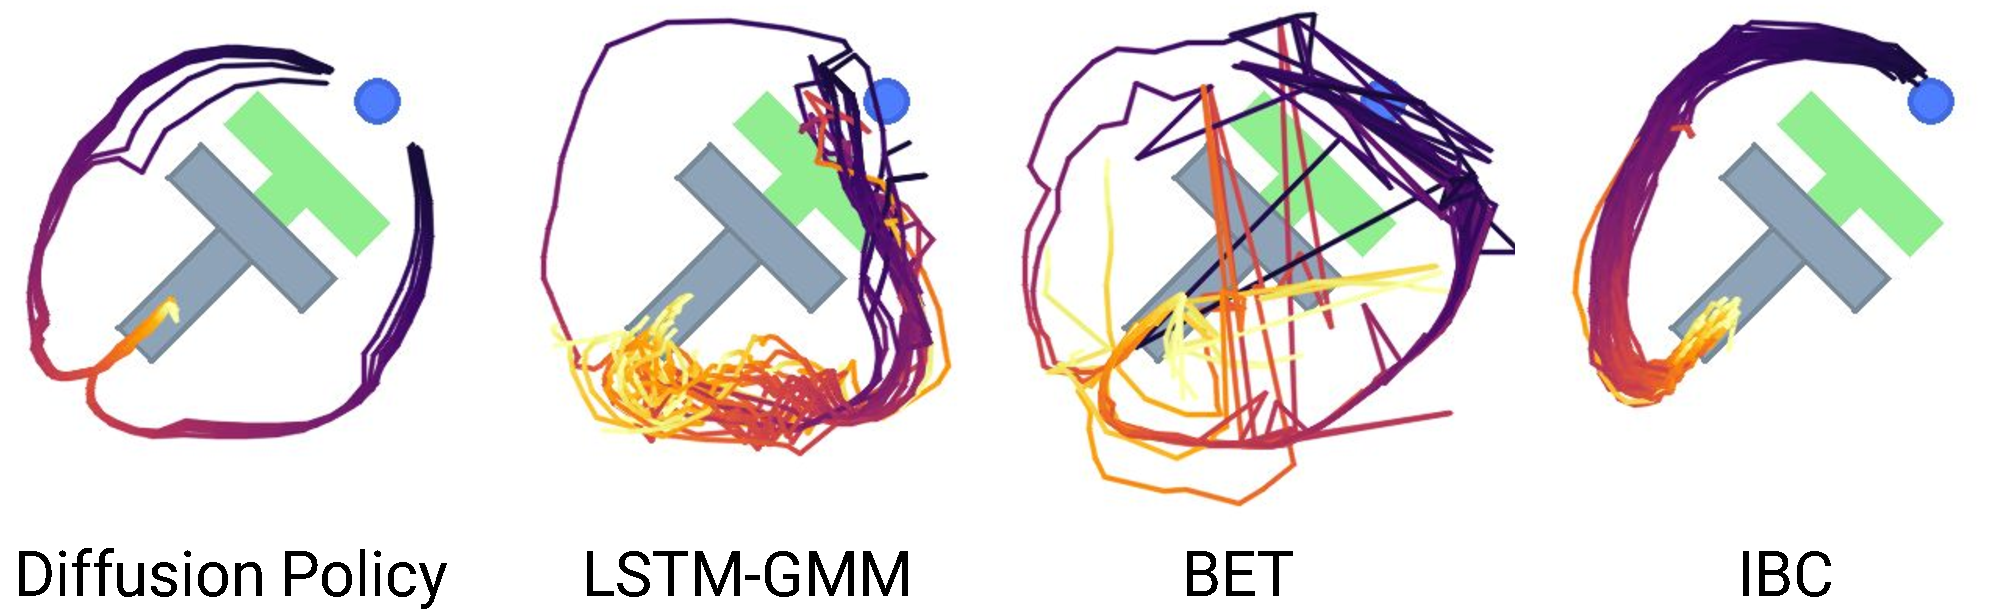
\includegraphics[width=0.98\linewidth]{figure/multimodal_sim.pdf} %

\caption{\label{fig:multimodal}
\textbf{Multimodal behavior.} At the given state, the end-effector (blue) can either go left or right to push the block.
\textbf{Diffusion Policy} learns both modes and commits to only one mode within each rollout.
In contrast, both \textbf{LSTM-GMM} \cite{robomimic} and \textbf{IBC} \cite{ibc} are biased toward one mode, while \textbf{BET} \cite{bet} fails to commit to a single mode due to its lack of temporal action consistency.
Actions generated by rolling out 40 steps for the best-performing checkpoint.
}
\vspace{-2mm}
\end{figure}
\subsection{Synergy with Position Control}
\label{sec:property_pos_vs_vel}
We find that Diffusion Policy with a position-control action space consistently outperforms Diffusion Policy with velocity control, as shown in Fig \ref{fig:pos_vs_vel}. This surprising result stands in contrast to the majority of recent behavior cloning work that generally relies on velocity control \cite{robomimic, bet, zhang2018deep, florence2019self, mandlekar2020learning, mandlekar2020iris}. We speculate that there are two primary reasons for this discrepancy: First, action multimodality is more pronounced in position-control mode than it is when using velocity control. Because Diffusion Policy better expresses action multimodality than existing approaches, we speculate that it is inherently less affected by this drawback than existing methods. Furthermore, position control suffers less than velocity control from compounding error effects and is thus more suitable for action-sequence prediction (as discussed in the following section). As a result, Diffusion Policy is both less affected by the primary drawbacks of position control and is better able to exploit position control's advantages.







\begin{figure}[h]
\centering
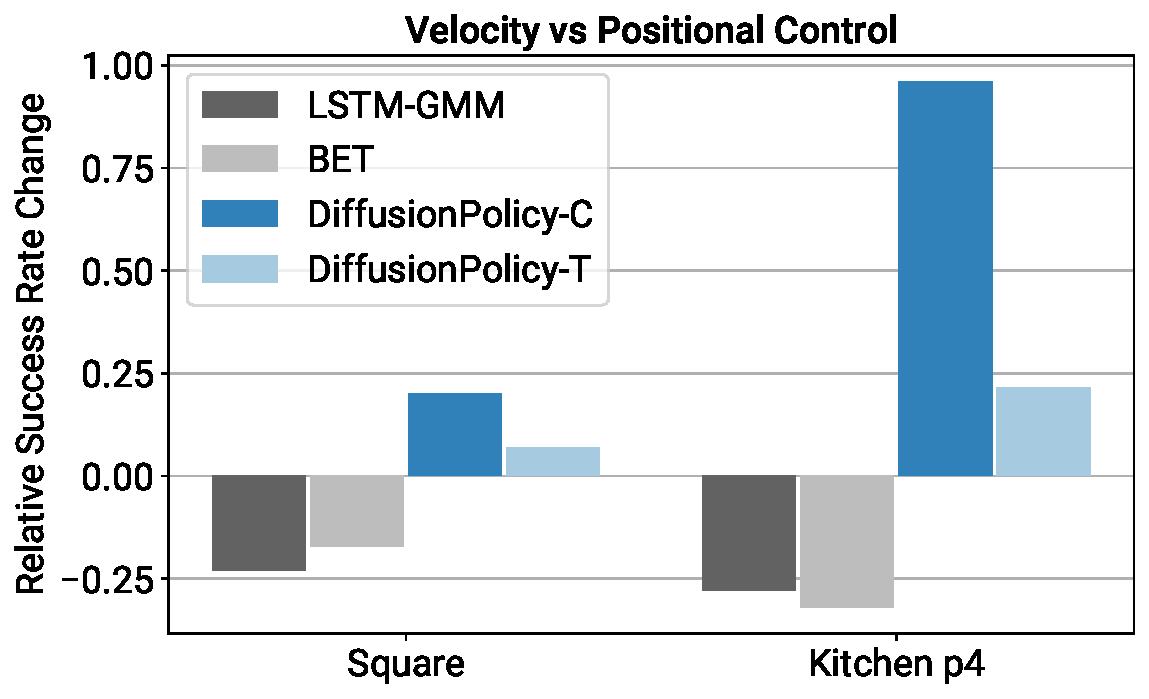
\includegraphics[width=0.85\linewidth]{figure/pos_vs_vel_figure.pdf}
\caption{\textbf{Velocity v.s. Position Control.} \label{fig:pos_vs_vel} The performance difference when switching from velocity to position control. While both BCRNN and BET performance decrease, Diffusion Policy is able to leverage the advantage of position and improve its performance. }
\vspace{-4mm}
\end{figure}



\subsection{Benefits of Action-Sequence Prediction}
\label{sec:action_sequence}



Sequence prediction is often avoided in most policy learning methods due to the difficulties in effectively sampling from high-dimensional output spaces. For example, IBC would struggle in effectively sampling high-dimensional action space with a non-smooth energy landscape. Similarly, BC-RNN and BET would have difficulty specifying the number of modes that exist in the action distribution (needed for GMM or k-means steps).

In contrast, DDPM scales well with output dimensions without sacrificing the expressiveness of the model, as demonstrated in many image generation applications. Leveraging this capability, Diffusion Policy represents action in the form of a high-dimensional action sequence, which naturally addresses the following issues:

\begin{itemize} [leftmargin=3mm]
    \item \textbf{Temporal action consistency}: Take Fig \ref{fig:multimodal} as an example. To push the T block into the target from the bottom, the policy can go around the T block from either left or right. However, suppose each action in the sequence is predicted as independent multimodal distributions (as done in BC-RNN and BET). In that case, consecutive actions could be drawn from different modes, resulting in jittery actions that alternate between the two valid trajectories.

    \item \textbf{Robustness to idle actions}: Idle actions occur when a demonstration is paused and results in sequences of identical positional actions or near-zero velocity actions. It is common during teleoperation and is sometimes required for tasks like liquid pouring. However, single-step policies can easily overfit to this pausing behavior. For example, BC-RNN and IBC often get stuck in real-world experiments when the idle actions are not explicitly removed from training.

\end{itemize}

\begin{figure}[h]
\centering
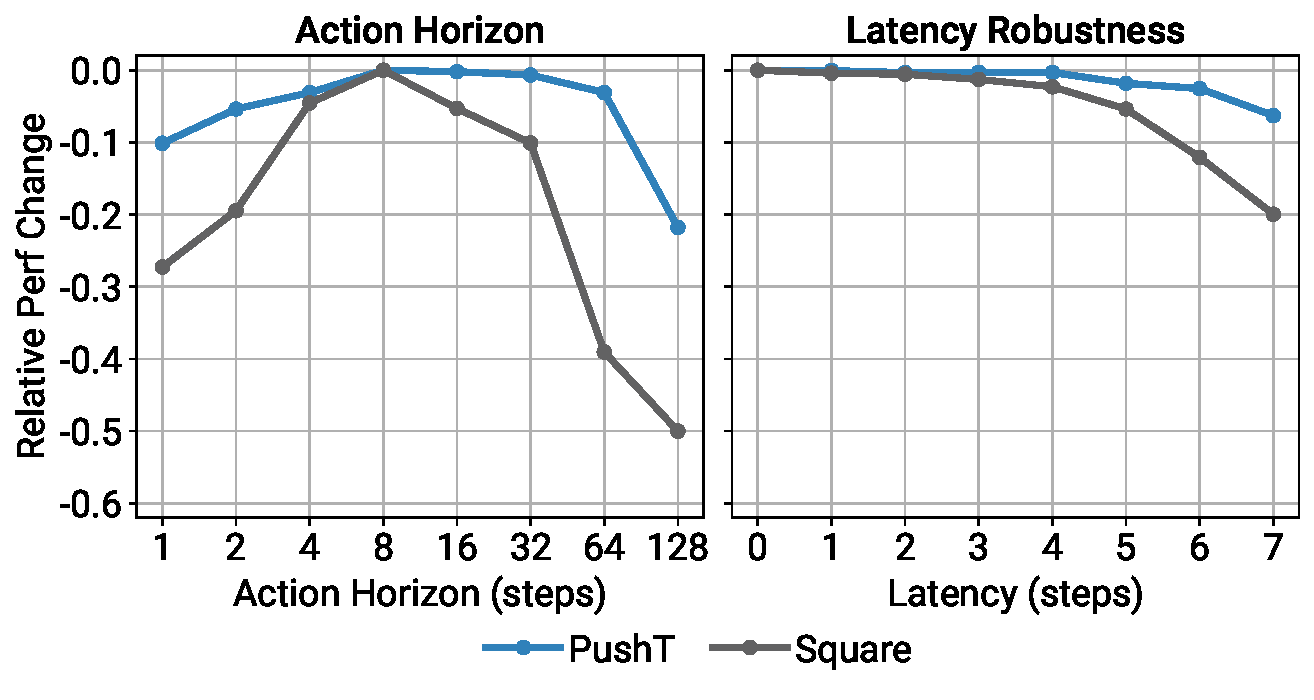
\includegraphics[width=\linewidth]{figure/ablation_figure.pdf}
\vspace{-6mm}

\caption{\textbf{Diffusion Policy Ablation Study.}
Change (difference) in success rate relative to the maximum for each task is shown on the Y-axis.
\textbf{Left}: trade-off between temporal consistency and responsiveness when selecting the action horizon.
\textbf{Right}: Diffusion Policy with position control is robust against latency.
Latency is defined as the number of steps between the last frame of observations to the first action that can be executed.
}
\label{fig:ablation}
\vspace{-5mm}
\end{figure}




\subsection{Training Stability}
\label{sec:ibc_stability}

While IBC, in theory, should possess similar advantages as diffusion policies. However, achieving reliable and high-performance results from IBC in practice is challenging due to IBC's inherent training instability \cite{ta2022conditional}. Fig \ref{fig:ibc_stability} shows training error spikes and unstable evaluation performance throughout the training process, making hyperparameter turning critical and checkpoint selection difficult. As a result, \citet{ibc} evaluate every checkpoint and report results for the best-performing checkpoint. In a real-world setting, this workflow necessitates the evaluation of many policies on hardware to select a final policy. Here, we discuss why Diffusion Policy appears significantly more stable to train.


An implicit policy represents the action distribution using an Energy-Based Model (EBM):
\vspace{-2mm}
\begin{equation}
    \label{eq:ebm}
    p_\theta(\mathbf{a}|\mathbf{o})=\frac{e^{-E_\theta(\mathbf{o},\mathbf{a})}}{Z(\mathbf{o},\theta)}
\vspace{-1mm}
\end{equation}
where $Z(\mathbf{o},\theta)$ is an intractable normalization constant (with respect to $\mathbf{a}$).

To train the EBM for implicit policy, an InfoNCE-style loss function is used, which equates to the negative log-likelihood of Eq \ref{eq:ebm}:
\begin{equation}
    \label{eq:infonce}
    \mathcal{L}_{infoNCE}=-\log(\frac{
        e^{-E_\theta(\mathbf{o},\mathbf{a})}
    }{
        e^{-E_\theta(\mathbf{o},\mathbf{a})} +
            \textcolor{red}{\sum^{N_{neg}}_{j=1}}e^{
                -E_\theta(\mathbf{o},\textcolor{red}{\widetilde{\mathbf{a}}^j})}
    })
\end{equation}
where a set of negative samples $\textcolor{red}{\{\widetilde{\mathbf{a}}^j\}^{N_{neg}}_{j=1}}$ are used to estimate the intractable normalization constant $Z(\mathbf{o},\theta)$. In practice, the inaccuracy of negative sampling is known to cause training instability for EBMs \cite{du2020improved,ta2022conditional}.

Diffusion Policy and DDPMs sidestep the issue of estimating $Z(\mathbf{a},\theta)$ altogether by modeling the \textbf{score function} \cite{song2019score} of the same action distribution in Eq \ref{eq:ebm}:
\begin{equation}
    \nabla_{\mathbf{a}}\log p(\mathbf{a}|\mathbf{o})
    =-\nabla_{\mathbf{a}} E_{\theta}(\mathbf{a},\mathbf{o})-\underbrace{\nabla_{\mathbf{a}}\log Z(\mathbf{o},\theta)}_{=0}
    \approx -\epsilon_\theta(\mathbf{a},\mathbf{o})
\end{equation}
where the noise-prediction network $\epsilon_\theta(\mathbf{a},\mathbf{o})$ is approximating the negative of the score function $\nabla_{\mathbf{a}}\log p(\mathbf{a}|\mathbf{o})$ \cite{liu2022compositional}, which is independent of the normalization constant $Z(\mathbf{o},\theta)$. As a result, neither the inference (Eq \ref{eq:diffusion_policy_langevin}) nor training (Eq \ref{eq:diffusion_policy_loss}) process of Diffusion Policy involves evaluating $Z(\mathbf{o},\theta)$, thus making Diffusion Policy training more stable.
\begin{figure}[h]
\centering
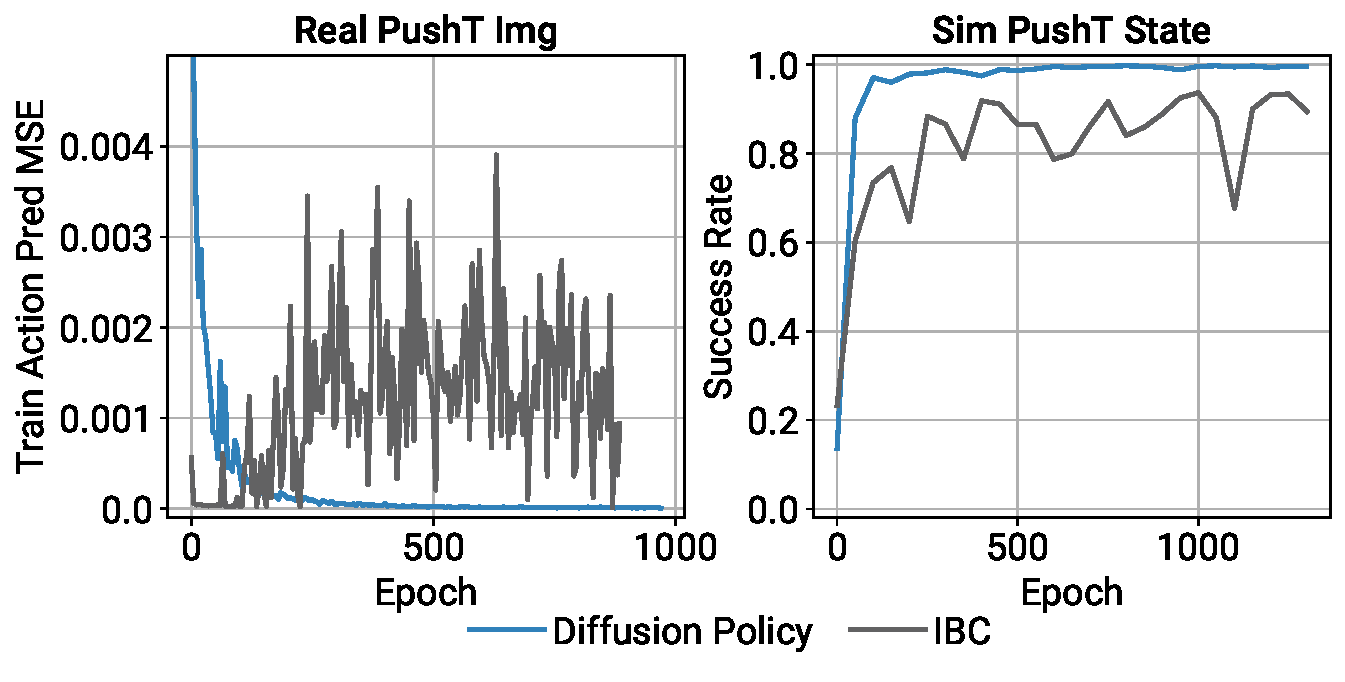
\includegraphics[width=\linewidth]{figure/ibc_stability_figure.pdf}
\vspace{-5mm}
\caption{\textbf{Training Stability.} \label{fig:ibc_stability}  Left: IBC fails to infer training actions with increasing accuracy despite smoothly decreasing training loss for energy function. Right: IBC's evaluation success rate oscillates, making checkpoint selection difficult (evaluated using policy rollouts in simulation).}

\end{figure}



\subsection{Connections to Control Theory}
\label{sec:control}
Diffusion Policy has a simple limiting behavior when the tasks are very simple; this potentially allows us to bring to bear some rigorous understanding from control theory. Consider the case where we have a linear dynamical system, in standard state-space form, that we wish to control:
\begin{gather*}
{\bf s}_{t+1} = {\bf A}{\bf s}_t + {\bf B}{\bf a}_t + {\bf w}_t, \qquad {\bf w}_t \sim \mathcal{N}(0, \Sigma_w).
\end{gather*} Now imagine we obtain demonstrations (rollouts) from a linear feedback policy: ${\bf a}_t = -{\bf K}{\bf s}_t.$ This policy could be obtained, for instance, by solving a linear optimal control problem like the Linear Quadratic Regulator. Imitating this policy does not need the modeling power of diffusion, but as a sanity check, we can see that Diffusion Policy does the right thing.

In particular, when the prediction horizon is one time step, $T_p=1$, it can be seen that the optimal denoiser which minimizes
\begin{equation}
    \mathcal{L}=MSE(\mathbf{\epsilon}^k,\epsilon_\theta(\mathbf{s}_t, -{\bf K}{\bf s}_t + \mathbf{\epsilon}^k, k))
\end{equation}
is given by $$\epsilon_\theta({\bf s}, {\bf a}, k) = \frac{1}{\sigma_k}[{\bf a} + {\bf K}{\bf s}],$$ where $\sigma_k$ is the variance on denoising iteration $k$. Furthermore, at inference time, the DDIM sampling will converge to the global minima at ${\bf a} = -{\bf Ks}.$

Trajectory prediction ($T_p>1$) follows naturally. In order to predict ${\bf a}_{t+t'}$ as a function of ${\bf s}_t$, the optimal denoiser will produce ${\bf a}_{t+t'} = -{\bf K}({\bf A}-{\bf BK})^{t'}{\bf s}_t$; all terms involving ${\bf w}_t$ are zero in expectation. This shows that in order to perfectly clone a behavior that depends on the state, the learner must implicitly learn a (task-relevant) dynamics model \cite{subramanian2019approximate,zhang2020learning}. Note that if either the plant or the policy is nonlinear, then predicting future actions could become significantly more challenging and once again involve multimodal predictions.

